As mentioned earlier, Autoware is based on ROS \cite{quigley2009ros},
\cite{rosorg}, which is a component-based middleware framework developed
for robotics research.
ROS is designed to enhance the modularity of robot applications at a
fine-grained level and is suitable for distributed systems, while
allowing for efficient development.
Since autonomous vehicles require many software packages, ROS provides a
strong foundation for Autoware's development.

In ROS, the software is abstracted as \emph{nodes} and \emph{topics}.
The \emph{nodes} represent individual component modules, whereas the \emph{topics} mediate inputs and outputs between \emph{nodes}, as illustrated in Figure \ref{fig:ros_pubsub}.
ROS \emph{nodes} are usually standard programs written in C++.
They can interface with any other software libraries that are installed.

Communication among \emph{nodes} follows a publish/subscribe model.
This model is a strong approach for modular development.
In this model, \emph{nodes} communicate by passing \emph{messages} via a \emph{topic}. 
A \emph{message} is structured simply (almost identical to structs in C) and is stored in .msg files.
\emph{Nodes} identify the content of the \emph{message} in terms of the \emph{topic} name.
When a \emph{node} publishes a \emph{message} to a \emph{topic}, another \emph{node} subscribes to the \emph{topic} and uses the \emph{message}. 
For example, in Figure \ref{fig:ros_pubsub}, the ``Camera Driver'' \emph{node} sends \emph{messages} to the ``Images'' \emph{topic}. 
The \emph{messages} in the \emph{topic} are received by the ``Traffic Light Recognition'' and ``Pedestrian Detection'' \emph{nodes}.
\emph{Topics} are managed using first-in, first-out queues when accessed by multiple \emph{nodes} simultaneously.
At the same time, ROS \emph{nodes} can launch several threads implicitly; however,
issues with real-time processing must be addressed.

ROS also includes an integrated visualization tool, RViz, and a
data-driven simulation tool, ROSBAG. 
Figure \ref{fig:rviz_autoware} (a) in Apendix B shows examples of visualizations produced by RViz for perception tasks in Autoware.
The RViz viewer is useful for monitoring the status of tasks.
ROSBAG is a set of tools for recording and playing back ROS \emph{topics}.
It provides development environments for testing self-driving algorithms without hardware, thereby making development processes more efficient.

\begin{figure*}[!htbp]
  \centering
  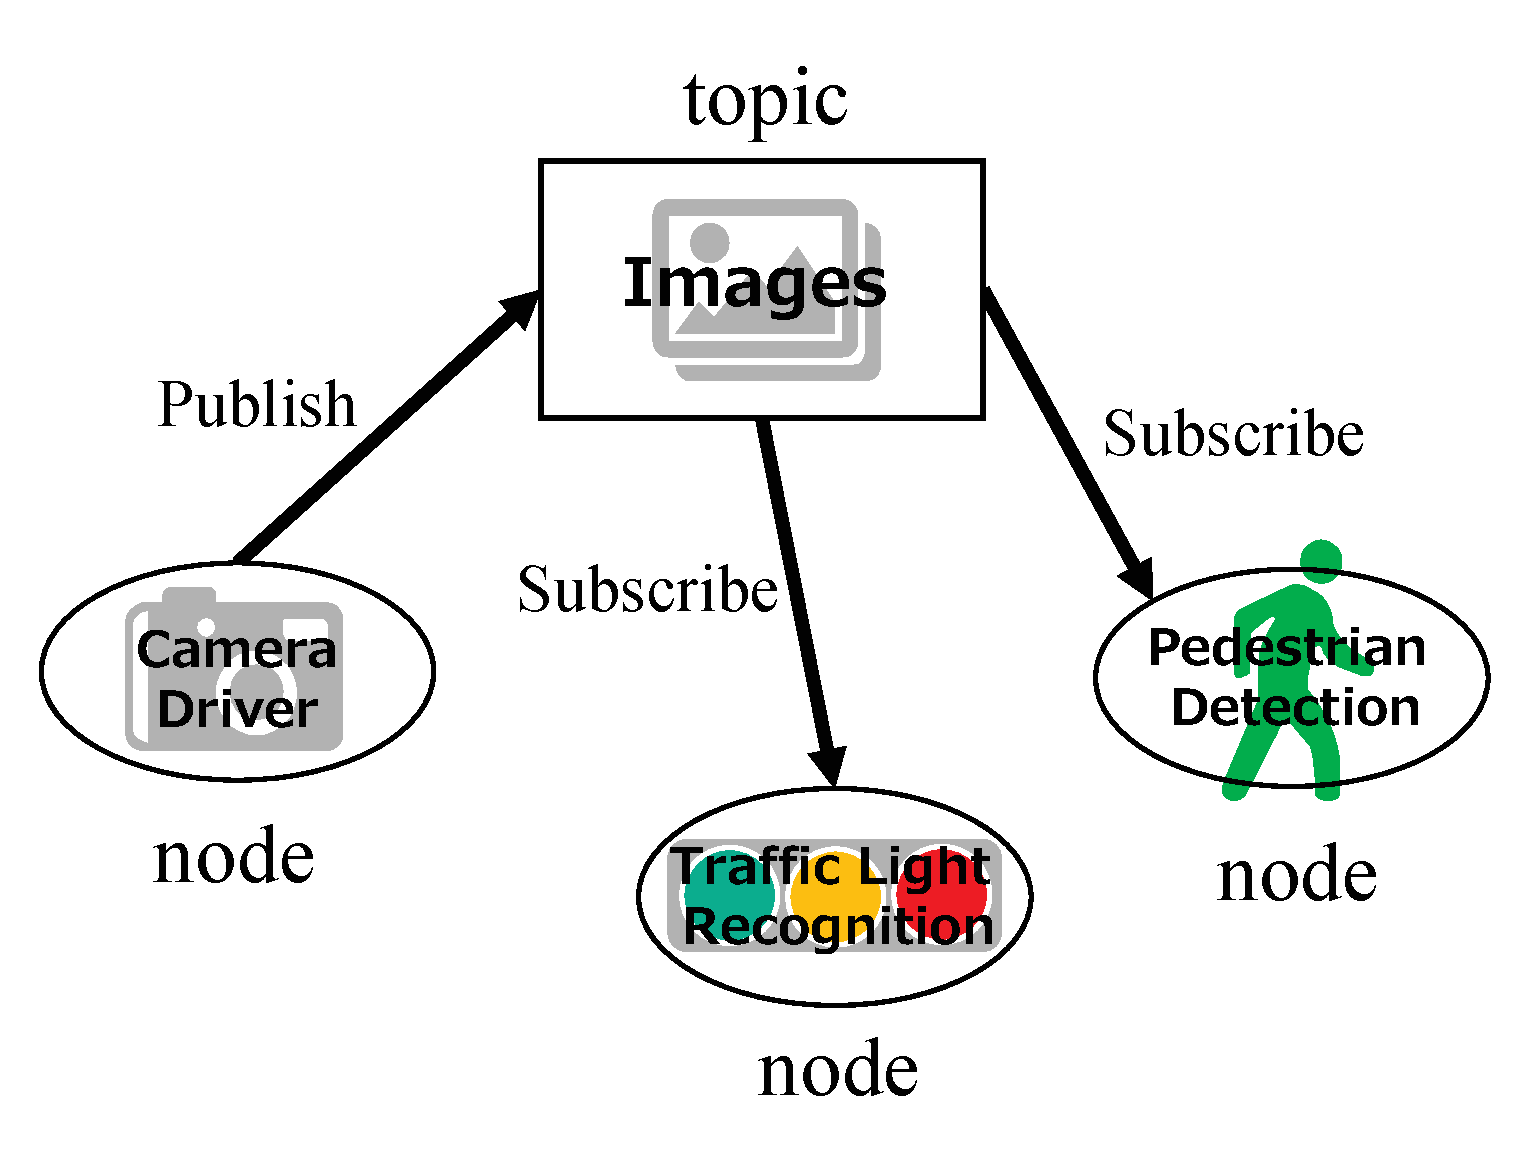
\includegraphics[width=0.8\linewidth]{../figure/ros_pubsub.eps}
  \caption{\label{fig:ros_pubsub}
 The publish/subscribe model in ROS.}
\end{figure*}

